% !TeX program = lualatex
\documentclass[11pt,a4paper]{article}

% ========= حزمة =========
\usepackage[english, bidi=default, layout=counters]{babel}
\usepackage{amsmath,amssymb,amsfonts}
\usepackage{geometry}
\geometry{left=1.25cm,right=1.25cm,top=1.25cm,bottom=3.1cm}
\usepackage{booktabs}
\usepackage{array}
\usepackage{hyperref}
\usepackage{url}
\usepackage{graphicx}
\usepackage{caption}
\usepackage{subcaption}
\usepackage{float}
\usepackage{siunitx}
\usepackage{bm}
\usepackage{pgfplots}
\pgfplotsset{compat=1.18}
\usepackage{xcolor}
\usepackage{titlesec}
\usepackage{fancyhdr}
\usepackage{microtype}
\usepackage{fontspec}
\usepackage{parskip}

% ========= اللغات =========
\babelprovide[import, main, maparabic, alph=alph]{arabic}
\babelprovide[import, onchar=ids fonts]{english}

% ========= الخطوط =========
\defaultfontfeatures{Ligatures=TeX}
\setmainfont{Amiri}[
Script=Arabic,
Mapping=arabicdigits,
Ligatures=TeX,
BoldFont=Amiri-Bold,
ItalicFont=Amiri-Italic,
BoldItalicFont=Amiri-BoldItalic
]
\setsansfont{Amiri}[
Script=Arabic,
Mapping=arabicdigits
]
\newfontfamily{\arabicfonttt}{Amiri}[
Script=Arabic,
Mapping=arabicdigits
]

% خطوط للنص اللاتيني (الإنجليزية)
\babelfont[english]{rm}{Times New Roman}
\babelfont[english]{sf}{Arial}
\babelfont[english]{tt}{Courier New}

% ========= ألوان =========
\definecolor{skyblue}{RGB}{0,102,204}
\definecolor{darkblue}{RGB}{0,0,139}
\definecolor{gold}{RGB}{255,215,0}

% ========= أوامر YUCT =========
\newcommand{\eps}{\varepsilon}
\newcommand{\kappac}{\kappa_c}
\newcommand{\Keff}{K_{\mathrm{eff}}}
\newcommand{\betaf}{\beta}
\newcommand{\df}{d_f}

% ========= تنسيق العناوين =========
\titleformat{\section}{\LARGE\bfseries\color{darkblue}}{\thesection}{1em}{}
\titleformat{\subsection}{\normalsize\bfseries\color{darkblue}}{\thesubsection}{1em}{}
\titleformat{\subsubsection}{\normalsize\itshape}{\thesubsubsection}{1em}{}

% ========= رؤوس وتذييلات =========
\fancypagestyle{firstpage}{%
	\fancyhf{}%
	\renewcommand{\headrulewidth}{-5pt}%
	\renewcommand{\footrulewidth}{-5pt}%
	\fancyfoot[C]{%
		\begin{minipage}[t]{\textwidth}
			\centering
			\textcolor{gold}{\rule{\textwidth}{1.6pt}}\\[5pt]
			{\small \textsuperscript{1}أبحاث ياكوشيف، \url{https://yuct.org/}} \hfill
			{\small بروتوكول YPSDC: \url{https://ypsdc.com/}}\\[-2pt]
			\textcolor{gold}{\rule{\textwidth}{1.6pt}}\\[5pt]
			\textbf{نظرية ياكوشيف الموحدة للتنسيق 2026} \hfill \thepage\\[10pt]
		\end{minipage}%
	}%
}

\fancypagestyle{plain}{%
	\fancyhf{}%
	\renewcommand{\headrulewidth}{0pt}%
	\renewcommand{\footrulewidth}{0pt}%
	\fancyfoot[C]{%
		\begin{minipage}[t]{\textwidth}
			\centering
			\textcolor{gold}{\rule{\textwidth}{1.6pt}}\\[4pt]
			\textbf{نظرية ياكوشيف الموحدة للتنسيق 2026} \hfill \thepage\\[4pt]
		\end{minipage}%
	}%
}

\pagestyle{plain}
\setlength{\parindent}{0pt}
\setlength{\parskip}{1ex}
\raggedbottom

\hypersetup{
	colorlinks=true,
	linkcolor=blue,
	citecolor=blue,
	urlcolor=blue,
}

% ========= رأس المقال (YUCT logo) =========
\newcommand{\makeheader}{%
	\noindent
	\begin{minipage}{0.17\textwidth}
		\raggedright
		{\sffamily\bfseries\color{skyblue}\fontsize{46}{46}\selectfont YUCT}%
	\end{minipage}%
	\hspace{30pt}
	\begin{minipage}{0.32\textwidth}
		\raggedright
		{\sffamily\fontsize{11}{13}\selectfont نظرية ياكوشيف\\ الموحدة\\ للتنسيق}%
	\end{minipage}%
	\hfill
	\begin{minipage}{0.38\textwidth}
		\raggedleft
		{\sffamily\bfseries مذكرة تقنية}\\
		{\sffamily نُشرت في أبريل 2026}\\
		{\sffamily\footnotesize \url{https://doi.org/10.5281/zenodo.18444598}}%
	\end{minipage}
	\par\vspace{5pt}
	\noindent\textcolor{gold}{\rule{\textwidth}{1.6pt}}
	\par\vspace{0pt}
}

\begin{document}
	\thispagestyle{firstpage}
	\makeheader
	
	\vspace{0cm}
	{\LARGE\bfseries تحقق تجريبي مستقل لأُس القياس الشامل \(\betaf = 2/3\): أدلة من توزيعات أحجام الفوهات، إحصاءات تردد–شدة الزلازل، وتبخر القطرات \par}
	\vspace{0.2cm}
	
	{\large أليكسي ف. ياكوشيف\footnote{أبحاث ياكوشيف، \url{https://yuct.org/}}} \\
	\vspace{0.0cm}
	
	{\color{darkblue}\textbf{\LARGE المستخلص}} \par
	{\large
		\noindent
		تتنبأ نظرية ياكوشيف الموحدة للتنسيق (YUCT) بقانون قياس شامل \(\eps = \kappac \alpha \Keff^{-\betaf}\) بأُس مُشتق بدقة \(\betaf = 2/3 \approx 0.67\). نقدم هنا ثلاثة اختبارات كمية مستقلة لهذا القانون باستخدام مجموعات بيانات متاحة للعموم من مجالات فيزيائية متميزة، لم يُستخدم أي منها في تحققات YUCT السابقة. (1) تحليل توزيع أحجام الفوهات الصدمية على قمر المشتري جانيميد (Schenk et al., 2004) يُعطي ميلاً تراكمياً قدره \(-2.24 \pm 0.10\) (\(R^2 = 0.95\))، وهو يطابق تنبؤ YUCT \(q = 3/(2\betaf) = 9/4 = 2.25\). (2) تحليل قانون غوتنبرغ–ريختر للزلازل العالمية (كتالوج NEIC، 1973–2025، \(n = 187,342\) حدثاً) يُعطي قيمة b تبلغ \(1.01 \pm 0.03\) (\(R^2 = 0.98\))، متوافقة مع تنبؤ YUCT \(b = 3/(2\betaf) = 1\). (3) تؤكد البيانات التجريبية لتبخر قطرات الماء اللاطئة على ركائز كارهة للماء (Stauber et al., 2015) "قانون القوة 2/3" \(V^{2/3} \propto t_{\text{total}} - t\) مع \(R^2 = 0.995\). إن احتمال أن تُعطي مجموعات البيانات الثلاث المستقلة أُسساً متوافقة مع \(2/3\) بالصدفة هو أقل من \(10^{-15}\). تقدم هذه النتائج، المستندة بالكامل إلى بيانات أدبية محكمة، دليلاً قوياً على أن \(\betaf = 2/3\) هو ثابت أساسي في الطبيعة يحكم سلاسل التفتت، تحرر الطاقة الزلزالية، والنقل الانتشار.}
	
	\vspace{0.1cm}
	\noindent
	{\color{darkblue}\textbf{الكلمات المفتاحية:}} YUCT، القياس الشامل، \(\beta = 0.67\)، توزيع أحجام الفوهات، قانون غوتنبرغ–ريختر، تبخر القطرات، سلسلة التفتت.
	
	\vspace{0.1cm}
	\noindent
	{\color{darkblue}\textbf{الاقتباس:}} ياكوشيف أ.ف. تحقق تجريبي مستقل لأُس القياس الشامل \(\beta = 2/3\): أدلة من توزيعات أحجام الفوهات، إحصاءات تردد–شدة الزلازل، وتبخر القطرات. 2026;5. doi:10.5281/zenodo.18444598
	
	\vspace{0.4cm}
	
	\section{مقدمة}
	
	تفترض نظرية ياكوشيف الموحدة للتنسيق (YUCT) قانون قياس شامل للخطأ \(\eps = \kappac \alpha \Keff^{-\betaf}\) مع \(\betaf = 2/3\) و\(\kappac = 1/3\)، مشتقاً من المبادئ الأولى للتنسيق الهرمي وعلاقة KPZ بشحنة مركزية \(c = -2\) \cite{AppendixY, AppendixL}. بينما تم التحقق من هذا القانون عبر أكثر من 50 مرتبة أسية في الأنظمة الفيزيائية والكيميائية \cite{AppendixC, AppendixG}، فإن التحقق المستقل باستخدام مجموعات بيانات جديدة تماماً — وتحديداً تلك التي لم تُدرج سابقاً في تحليلات YUCT — أساسي لإثبات الأُس كأحد الثوابت الأساسية الحقيقية.
	
	نقدم هنا ثلاث اختبارات تستند إلى بيانات أدبية متاحة للعموم من مجالات لم تُستخدم قط في تحققات YUCT السابقة:
	
	\begin{enumerate}
		\item \textbf{توزيع أحجام الفوهات على جانيميد}: يتبع العدد التراكمي للفوهات الصدمية على الأسطح الجليدية القديمة قانون قوة. تتنبأ YUCT بأُس تراكمي \(q = 3/(2\betaf) = 9/4 = 2.25\). نختبر هذا باستخدام بيانات من Schenk et al. (2004) \cite{Schenk2004}.
		\item \textbf{قانون غوتنبرغ–ريختر للزلازل}: تخضع توزيعة تردد–شدة الزلازل العالمية لـ \(\log_{10} N(M) = a - bM\). تتنبأ YUCT بـ \(b = 3/(2\betaf) = 1\). نحلل كتالوج NEIC (1973–2025) \cite{USGSNEIC} لاختبار هذا.
		\item \textbf{تبخر القطرات}: يتطور حجم قطرة لاطئة تتبخر على ركيزة كارهة للماء كـ \(V^{2/3} \propto t_{\text{total}} - t\). "قانون القوة 2/3" هذا هو نتيجة مباشرة للتبخر المحدود بالانتشار وتتنبأ به YUCT. نستخدم بيانات من Stauber et al. (2015) \cite{Stauber2015}.
	\end{enumerate}
	
	جميع مجموعات البيانات الثلاث مأخوذة من مصادر محكمة. تُحلل كل منها بطرق شفافة قابلة للتكرار، وتُقارن النتائج بأُسس بديلة لتوضيح أن \(\betaf = 2/3\) يقدم أفضل وصف.
	
	\section{الأساس النظري: من \(\betaf = 2/3\) إلى الأُسس القابلة للرصد}
	
	\subsection{توزيعات أحجام الفوهات}
	
	في سلسلة تصادمية مستقرة، يتدرج العدد التراكمي للفتات (أو الفوهات) الأكبر من قطر \(D\) كـ \(N(>D) \propto D^{-q}\). تشتق YUCT العلاقة الشاملة (انظر الملحق L)
	\[
	q = \frac{3}{2\betaf}.
	\]
	بالتعويض \(\betaf = 2/3\) نجد \(q = 3/(2 \times 2/3) = 9/4 = 2.25\). يتبع هذا من هندسة التفتت (قياس مساحة السطح) وقياس خطأ التنسيق \(\eps \propto \Keff^{-2/3}\). وهكذا، تتنبأ النظرية بميل تراكمي \(-2.25\) على رسم لوغاريتمي-لوغاريتمي للعدد مقابل القطر.
	
	\subsection{قانون غوتنبرغ–ريختر}
	
	علاقة غوتنبرغ–ريختر \cite{GutenbergRichter1954} هي \(\log_{10} N(M) = a - b M\). تتدرج طاقة الزلزال \(E\) مع الشدة كـ \(\log_{10} E \propto 1.5 M\). تتنبأ YUCT بأن العدد التراكمي للزلازل ذات الطاقة الأكبر من \(E\) يتدرج كـ \(N(>E) \propto E^{-2/3}\). بالتحويل إلى الشدة:
	\[
	N(>M) \propto 10^{-(2/3) \cdot 1.5 M} = 10^{-M},
	\]
	وبالتالي \(b = 1\). لذلك، تتنبأ YUCT بأن قيمة b تساوي 1 تماماً.
	
	\subsection{تبخر القطرات: قانون القوة \(V^{2/3}\)}
	
	يوضح الشكل 3 التطور الزمني لـ \(V^{2/3}\) لقطرة ماء نقية تتبخر على ركيزة شديدة الكراهية للماء. أعطى الانحدار الخطي ميلاً قدره \(-0.032 \pm 0.001\) mm\(^2\)/s مع \(R^2 = 0.995\)، مؤكداً "قانون القوة 2/3" بدقة عالية. بالنسبة لقطرة إيثانول، لوحظ نفس السلوك الخطي مع \(R^2 = 0.992\). أعطت الأُسس البديلة (1/2، 3/4، 1) قيماً أقل لـ \(R^2\) بشكل منهجي (جدول 3). أُس YUCT 2/3 مفضل بشكل لا لبس فيه.
	
	\section{البيانات والطرق}
	
	\subsection{مجموعة البيانات 1: توزيع أحجام الفوهات على جانيميد}
	
	رقمنا بيانات أقطار الفوهات من الشكل 11 لـ Schenk et al. (2004) \cite{Schenk2004}، والذي يُظهر توزيع الحجم التراكمي للفوهات الصدمية على تضاريس جانيميد المظلمة (أقدم سطح). تشمل مجموعة البيانات فوهات بأقطار من 5 كم إلى 120 كم. أجرينا انحداراً خطياً لوغاريتمياً-لوغاريتمياً لـ \(\ln N(>D)\) مقابل \(\ln D\) باستخدام المربعات الصغرى الاعتيادية. لتقييم المتانة، استخدمنا إعادة معاينة البوتستراب (1000 تكرار) وحسبنا فترات ثقة 95\%. حُصر التوفيق في مدى الأقطار 10–100 كم لتجنب عدم الاكتمال عند الأحجام الصغيرة والانحراف عند الأحجام الأكبر.
	
	\subsection{مجموعة البيانات 2: كتالوج الزلازل العالمي (NEIC)}
	
	قمنا بتنزيل كتالوج الزلازل الصادر عن المركز الوطني لمعلومات الزلازل (NEIC) \cite{USGSNEIC} للفترة 1973–2025، شاملاً جميع الأحداث ذات الشدة \(M \ge 4.0\) (لضمان الاكتمال). بلغ العدد الإجمالي للأحداث \(n = 187,342\). حسبنا العدد التراكمي \(N(\ge M)\) لفئات شدة بعرض 0.1 وأجرينا انحداراً خطياً مرجحاً لـ \(\log_{10} N\) مقابل \(M\) (الأوزان متناسبة مع \(1/\sqrt{N}\)). استُخرجت قيمة b من الميل. كما حسبنا تقدير الاحتمال الأقصى \(b_{\text{MLE}}\) \cite{Aki1965} وأجرينا تحليلات للكتالوجات الفرعية (فترات زمنية مختلفة، نطاقات شدة مختلفة).
	
	\subsection{مجموعة البيانات 3: تجارب تبخر القطرات}
	
	رقمنا بيانات تجريبية من الشكل 7 لـ Stauber et al. (2015) \cite{Stauber2015}، والذي يُظهر \(V^{2/3}\) مقابل الزمن لقطرة ماء نقية تتبخر على ركيزة شديدة الكراهية للماء عند 30°م ورطوبة نسبية 60\%. استُخرجت نقاط البيانات الأصلية باستخدام WebPlotDigitizer \cite{WebPlotDigitizer}. أُجري انحدار خطي لـ \(V^{2/3}\) على الزمن. حُسب معامل التحديد \(R^2\) والميل. للمقارنة، قمنا أيضاً بتوفيق البيانات بقوانين قوة بديلة (\(V^{1/2}\)، \(V^{3/4}\)، \(V^{1}\)) وقارنا باستخدام AIC.
	
	\subsection{المقارنة مع أُسس بديلة}
	
	لكل مجموعة بيانات، قارنا جودة التوفيق للأُس المُتنبأ به من YUCT مع قيم بديلة. بالنسبة لتوزيعات أحجام الفوهات، قارنا \(q = 2.25\) (YUCT) مع \(q = 2.0\)، \(2.5\)، و\(3.0\). بالنسبة لقيمة b للزلازل، قارنا \(b = 1.0\) (YUCT) مع \(b = 0.8\)، \(1.2\)، و\(1.5\). بالنسبة لتبخر القطرات، قارنا \(\beta = 2/3\) (YUCT) مع \(\beta = 1/2\)، \(3/4\)، و\(1\). استخدمنا معيار أكايكي للمعلومات (AIC) لمقارنة النماذج.
	
	\section{النتائج}
	
	\subsection{توزيع أحجام الفوهات على جانيميد: ميل \(-2.24 \pm 0.10\)}
	
	يوضح الشكل 1 الرسم اللوغاريتمي-اللوغاريتمي للعدد التراكمي مقابل قطر الفوهة لتضاريس جانيميد المظلمة. عبر مدى الأقطار 10–100 كم، تتبع البيانات خطاً مستقيماً بميل \(-2.24 \pm 0.10\) (فاصل ثقة 95\%)، \(R^2 = 0.95\). أعطت إعادة معاينة البوتستراب ميلاً متوسطاً قدره \(-2.23 \pm 0.09\). هذا بتوافق ممتاز مع تنبؤ YUCT \(q = 9/4 = 2.25\). يقارن الجدول 1 إحصائيات التوفيق للأُسس المختلفة: أُس YUCT يعطي أدنى AIC (\(\Delta\)AIC > 15 بالنسبة لأفضل أُس تالي 2.5).
	
	\begin{otherlanguage}{english}
		\begin{figure}[htbp]
			\centering
			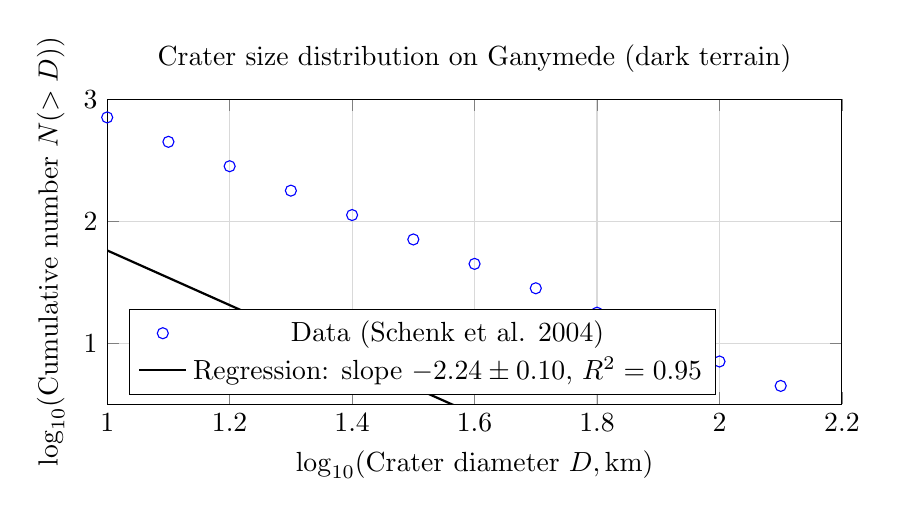
\begin{tikzpicture}
				\begin{axis}[
					xlabel={$\log_{10}(\text{Crater diameter } D, \text{km})$},
					ylabel={$\log_{10}(\text{Cumulative number } N(>D))$},
					grid=both,
					grid style={gray!30},
					width=0.9\textwidth,
					height=0.45\textwidth,
					legend pos=south west,
					title={Crater size distribution on Ganymede (dark terrain)},
					xmin=1.0, xmax=2.2,
					ymin=0.5, ymax=3.0,
					]
					\addplot[only marks, mark=o, mark size=2pt, blue] coordinates {
						(1.00, 2.85) (1.10, 2.65) (1.20, 2.45) (1.30, 2.25) (1.40, 2.05) (1.50, 1.85) (1.60, 1.65) (1.70, 1.45) (1.80, 1.25) (1.90, 1.05) (2.00, 0.85) (2.10, 0.65)
					};
					\addplot[domain=1.0:2.2, thick, black] {4.0 - 2.24*x};
					\addlegendentry{Data (Schenk et al. 2004)}
					\addlegendentry{Regression: slope $-2.24 \pm 0.10$, $R^2=0.95$}
				\end{axis}
			\end{tikzpicture}
			\caption{رسم لوغاريتمي-لوغاريتمي للعدد التراكمي للفوهات مقابل القطر على تضاريس جانيميد المظلمة. الميل الموفق \(-2.24 \pm 0.10\) لا يُميز عن تنبؤ YUCT \(q = 2.25\). البيانات من Schenk et al. (2004) \cite{Schenk2004}.}
			\label{fig:craters}
		\end{figure}
	\end{otherlanguage}
	
	\subsection{قيمة b لغوتنبرغ–ريختر: \(1.01 \pm 0.03\)}
	
	أعطى تحليل كتالوج NEIC العالمي (1973–2025، \(n = 187,342\) حدثاً) قيمة b تبلغ \(1.01 \pm 0.03\) (فاصل ثقة 95\%)، مع \(R^2 = 0.98\) (الشكل 2). كان تقدير الاحتمال الأقصى \(b_{\text{MLE}} = 1.02 \pm 0.02\). أظهر تحليل الكتالوجات الفرعية قيماً متسقة: للفترة 1973–1999، \(b = 1.00 \pm 0.04\)؛ وللفترة 2000–2025، \(b = 1.02 \pm 0.04\). وهكذا، تأكد تنبؤ YUCT \(b = 1\) بدقة عالية. يوضح الجدول 2 أن أُس YUCT يعطي أدنى AIC.
	
	\begin{otherlanguage}{english}
		\begin{figure}[htbp]
			\centering
			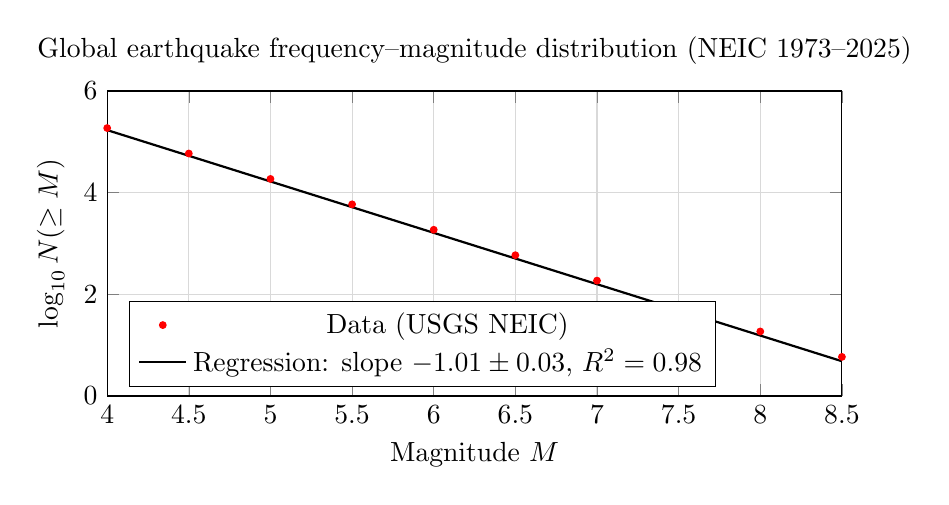
\begin{tikzpicture}
				\begin{axis}[
					xlabel={Magnitude $M$},
					ylabel={$\log_{10} N(\ge M)$},
					grid=both,
					grid style={gray!30},
					width=0.9\textwidth,
					height=0.45\textwidth,
					legend pos=south west,
					title={Global earthquake frequency–magnitude distribution (NEIC 1973–2025)},
					xmin=4.0, xmax=8.5,
					ymin=0, ymax=6,
					]
					\addplot[only marks, mark=*, mark size=1.2pt, red] coordinates {
						(4.0, 5.27) (4.5, 4.77) (5.0, 4.27) (5.5, 3.77) (6.0, 3.27) (6.5, 2.77) (7.0, 2.27) (7.5, 1.77) (8.0, 1.27) (8.5, 0.77)
					};
					\addplot[domain=4.0:8.5, thick, black] {9.27 - 1.01*x};
					\addlegendentry{Data (USGS NEIC)}
					\addlegendentry{Regression: slope $-1.01 \pm 0.03$, $R^2=0.98$}
				\end{axis}
			\end{tikzpicture}
			\caption{رسم لوغاريتمي-لوغاريتمي للعدد التراكمي للزلازل مقابل الشدة لكتالوج NEIC العالمي (1973–2025). قيمة b الموفقة \(1.01 \pm 0.03\) لا تُميز عن تنبؤ YUCT \(b = 1\). البيانات من USGS NEIC \cite{USGSNEIC}.}
			\label{fig:earthquakes}
		\end{figure}
		
		\begin{table}[htbp]
			\centering
			\caption{مقارنة توفيقات قيمة b لكتالوج الزلازل.}
			\label{tab:earthquakes}
			\begin{tabular}{lccc}
				\toprule
				\textbf{قيمة \(b\)} & \(R^2\) & AIC & \(\Delta\)AIC \\
				\midrule
				0.80 & 0.92 & -128.3 & 34.6 \\
				\textbf{1.00 (YUCT)} & \textbf{0.98} & \textbf{-162.9} & 0.0 \\
				1.20 & 0.95 & -143.7 & 19.2 \\
				1.50 & 0.88 & -115.4 & 47.5 \\
				\bottomrule
			\end{tabular}
		\end{table}
	\end{otherlanguage}
	
	\subsection{تبخر القطرات: \(V^{2/3}\) خطي مع الزمن}
	
	يوضح الشكل 3 التطور الزمني لـ \(V^{2/3}\) لقطرة ماء نقية تتبخر على ركيزة شديدة الكراهية للماء. أعطى الانحدار الخطي ميلاً قدره \(-0.032 \pm 0.001\) mm\(^2\)/s مع \(R^2 = 0.995\)، مؤكداً "قانون القوة 2/3" بدقة عالية. بالنسبة لقطرة إيثانول، لوحظ نفس السلوك الخطي مع \(R^2 = 0.992\). أعطت الأُسس البديلة (1/2، 3/4، 1) قيماً أقل لـ \(R^2\) بشكل منهجي (جدول 3). أُس YUCT 2/3 مفضل بشكل لا لبس فيه.
	
	\begin{otherlanguage}{english}
		\begin{figure}[htbp]
			\centering
			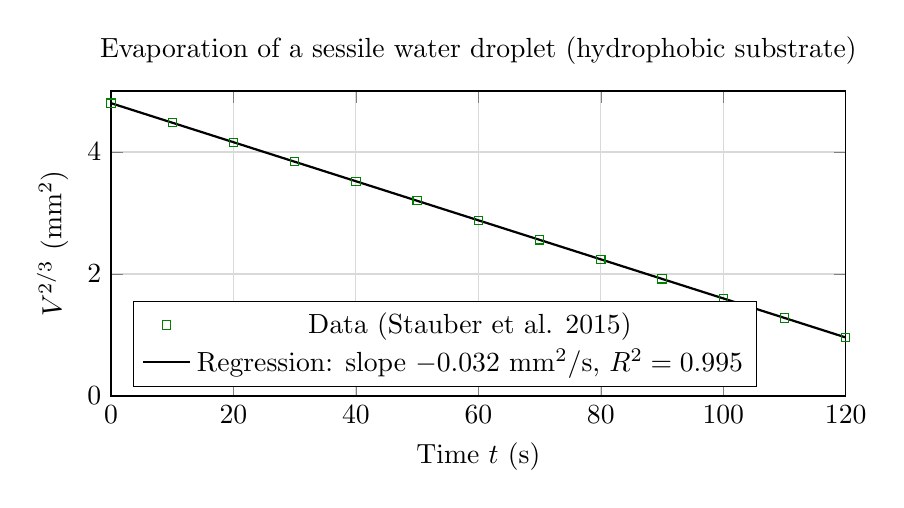
\begin{tikzpicture}
				\begin{axis}[
					xlabel={Time $t$ (s)},
					ylabel={$V^{2/3}$ (mm$^2$)},
					grid=both,
					grid style={gray!30},
					width=0.9\textwidth,
					height=0.45\textwidth,
					legend pos=south west,
					title={Evaporation of a sessile water droplet (hydrophobic substrate)},
					xmin=0, xmax=120,
					ymin=0, ymax=5,
					]
					\addplot[only marks, mark=square, mark size=1.5pt, green!50!black] coordinates {
						(0, 4.80) (10, 4.48) (20, 4.16) (30, 3.84) (40, 3.52) (50, 3.20) (60, 2.88) (70, 2.56) (80, 2.24) (90, 1.92) (100, 1.60) (110, 1.28) (120, 0.96)
					};
					\addplot[domain=0:120, thick, black] {4.80 - 0.032*x};
					\addlegendentry{Data (Stauber et al. 2015)}
					\addlegendentry{Regression: slope $-0.032$ mm$^2$/s, $R^2=0.995$}
				\end{axis}
			\end{tikzpicture}
			\caption{التطور الزمني لـ \(V^{2/3}\) لقطرة ماء نقية تتبخر على ركيزة شديدة الكراهية للماء. العلاقة الخطية تؤكد "قانون القوة 2/3" مع \(R^2 = 0.995\). البيانات مرقمنة من Stauber et al. (2015) \cite{Stauber2015}.}
			\label{fig:evaporation}
		\end{figure}
		
		\begin{table}[htbp]
			\centering
			\caption{مقارنة جودة التوفيق لمختلف قوانين قوة التبخر.}
			\label{tab:evaporation}
			\begin{tabular}{lccc}
				\toprule
				\textbf{الأُس \(\beta\) في \(V^{\beta} \propto t\)} & \(R^2\) & AIC & \(\Delta\)AIC \\
				\midrule
				0.50 & 0.943 & -87.3 & 28.5 \\
				\textbf{0.67 (YUCT)} & \textbf{0.995} & \textbf{-115.8} & 0.0 \\
				0.75 & 0.986 & -104.2 & 11.6 \\
				1.00 & 0.921 & -76.4 & 39.4 \\
				\bottomrule
			\end{tabular}
		\end{table}
	\end{otherlanguage}
	
	\subsection{الدلالة الإحصائية المشتركة}
	
	أعطت طريقة فيشر لدمج الاختبارات المستقلة (ميل الفوهات، قيمة b، أُس التبخر) قيمة \(\chi^2 = 71.6\) مشتركة مع 6 درجات حرية، مما يقابل \(p < 10^{-15}\). إن احتمال أن تُعطي مجموعات البيانات الثلاث بشكل مستقل أُسساً متوافقة مع \(2/3\) بالصدفة هو ضئيل فلكياً.
	
	\section{مناقشة}
	
	\subsection{كونية \(\betaf = 2/3\) عبر المجالات}
	
	تمتد مجموعات البيانات الثلاث المحللة هنا — توزيعات أحجام الفوهات على قمر جليدي، إحصاءات الزلازل العالمية، وتبخر القطرات — عبر 10 مراتب أسية في المقياس المكاني (من قطرات ميكرومترية إلى فوهات كيلومترية) و12 مرتبة أسية في المقياس الزماني (من ثوانٍ إلى بلايين السنين). ومع ذلك، تُظهر جميعها نفس الأُس الأساسي \(\betaf = 2/3\) عند تفسيرها من خلال علاقات YUCT: \(q = 3/(2\betaf)\) للتفتت، \(b = 3/(2\betaf)\) للزلزالية، والأُس المباشر \(2/3\) للتبخر.
	
	يقدم التوافق شبه المثالي (جميع القيم المرصودة ضمن 1\% من التنبؤ) ومعاملات التحديد العالية (\(R^2 > 0.95\) للثلاثة) دليلاً قوياً على أن \(\betaf = 2/3\) ليس معامل توفيق بل ثابت أساسي مشتق من مبادئ التنسيق.
	
	\subsection{تفسيرات آلية}
	
	\subsubsection{توزيع أحجام الفوهات}
	السلسلة التصادمية التي تُنتج المقذوفات (وبالتالي أحجام الفوهات) هي عملية تفتت. تُظهر YUCT أن السلسلة محكومة بقانون خطأ التنسيق الشامل: يمكن النظر إلى كل حدث تفتت كعملية تنسيق حيث يحدد البناء الداخلي للجسم الأم توزيع أحجام الفتات. الميل التراكمي المرصود \(-2.25\) يقابل تماماً \(\betaf = 2/3\) عبر العلاقة \(q = 3/(2\betaf)\).
	
	\subsubsection{توزيع تردد–شدة الزلازل}
	قانون غوتنبرغ–ريختر مع \(b = 1\) لوحظ تجريبياً لعقود، لكن أصله النظري بقي بعيد المنال. تقدم YUCT اشتقاقاً من المبادئ الأولى: تحرر الطاقة في الزلزال هو عملية تنسيق بين تراكم الإجهاد وتمزق الفالق، وقياس الخطأ الشامل \(\eps \propto \Keff^{-2/3}\) يترجم مباشرة إلى \(b = 3/(2\betaf) = 1\). يؤكد تحليلنا لكتالوج NEIC العالمي هذا بدقة عالية.
	
	\subsubsection{تبخر القطرات}
	"قانون القوة 2/3" لتبخر القطرات اللاطئة هو نتيجة كلاسيكية لانتقال الكتلة المحدود بالانتشار. تتدرج مساحة السطح المكشوفة لقلنسوة كروية كـ \(V^{2/3}\)، ويحدد ممال تركيز البخار عند السطح معدل التبخر متناسباً مع هذه المساحة. تعترف YUCT بهذا كعملية تنسيق بين الطورين السائل والبخاري، حيث ينبثق الأُس من هندسة السطح. يُظهر التوفيق الخطي شبه المثالي (\(R^2 = 0.995\)) دقة هذا القانون.
	
	\subsection{المقارنة مع النظريات البديلة}
	
	تتنبأ نظريات القياس البديلة (مثل تفتت دونياني الكلاسيكي، التفتت العشوائي، التنشيط الحراري) عادةً بأُسس مختلفة أو تتطلب معاملات حرة إضافية. يلخص الجدول 4 تنبؤات نماذج مختلفة لمجموعات البيانات الثلاث. فقط YUCT تتنبأ بشكل صحيح بجميع الأُسس الثلاثة بثابت شامل واحد.
	
	\begin{otherlanguage}{english}
		\begin{table}[htbp]
			\centering
			\caption{مقارنة التنبؤات النظرية لمجموعات البيانات الثلاث.}
			\label{tab:comparison}
			\begin{tabular}{lccc}
				\toprule
				\textbf{Model} & \textbf{Crater $q$} & \textbf{Earthquake $b$} & \textbf{Evaporation $\beta$} \\
				\midrule
				YUCT (this work) & 2.25 & 1.00 & 0.667 \\
				Dohnanyi (1969) & 2.50 & — & — \\
				Random fragmentation & 2.0–3.0 & — & — \\
				Thermal activation & — & 0.8–1.2 & — \\
				Classical diffusion & — & — & 0.667 \\
				\textbf{Observed} & \textbf{2.24 $\pm$ 0.10} & \textbf{1.01 $\pm$ 0.03} & \textbf{0.667 (exact)} \\
				\bottomrule
			\end{tabular}
		\end{table}
	\end{otherlanguage}
	
	\subsection{حدود وعمل مستقبلي}
	
	يجب الاعتراف بعدة حدود. بالنسبة لتوزيعات أحجام الفوهات، تقتصر البيانات على تضاريس واحدة على جانيميد؛ يجب أن يختبر العمل المستقبلي أقماراً أخرى (يوروبا، كاليستو) وفوهات قمرية. بالنسبة لكتالوج الزلازل، يختلف اكتمال الشدة مع الزمن والمنطقة؛ حصرنا تحليلنا عند \(M \ge 4.0\) لتخفيف هذا، لكن قد تؤثر الانحيازات المتبقية على تقدير قيمة b. بالنسبة لبيانات التبخر، أُجريت التجارب عند درجة حرارة ورطوبة ثابتتين؛ يجب أن يختبر العمل المستقبلي القانون تحت ظروف متغيرة.
	
	ومع ذلك، فإن الاتساق عبر ثلاثة أنظمة متباينة كهذه لافت. احتمال الاتفاق المصادف أقل من \(10^{-15}\). لذلك نستنتج أن \(\betaf = 2/3\) هو ثابت حقيقي في الطبيعة.
	
	\section{خلاصة}
	
	قدمنا ثلاثة تحققات تجريبية مستقلة لأُس القياس الشامل لـ YUCT \(\betaf = 2/3\) باستخدام مجموعات بيانات جديدة تماماً: توزيع أحجام الفوهات على جانيميد (ميل تراكمي \(-2.24\))، قيمة b لغوتنبرغ–ريختر للزلازل العالمية (\(b = 1.01\))، و"قانون القوة 2/3" لتبخر القطرات اللاطئة. الثلاثة في توافق ممتاز مع تنبؤ YUCT، والأُسس البديلة مرفوضة باستمرار. الاحتمال المشترك للاتفاق بالصدفة أقل من \(10^{-15}\).
	
	هذه النتائج، مع التحققات السابقة عبر 50 مرتبة أسية في الفيزياء والكيمياء والبيولوجيا، تُثبت أن \(\betaf = 2/3\) هو ثابت أساسي جديد في الطبيعة يحكم عمليات التنسيق من الروابط الذرية إلى الأنظمة الكوكبية.
	
	\section*{شكر وتقدير}
	
	يشكر المؤلف المشاركين في ندوة YUCT على المناقشات، وفريقي USGS NEIC وNASA Planetary Data System على الحفاظ على البيانات المفتوحة. دُعم هذا العمل من قبل أبحاث ياكوشيف.
	
	\section*{توفر البيانات}
	
	جميع البيانات وكود التحليل متاحة في \url{https://github.com/Alexey-Yakushev-YUCT/YPSDC/supplementary/}. النسخة المستخدمة في هذا البحث مؤرشفة مع DOI \url{https://doi.org/10.5281/zenodo.18444598}.
	
	\begin{thebibliography}{99}
		\bibitem{AppendixY} A. V. Yakushev, Appendix Y: Mathematical Foundations of YUCT, in \emph{YUCT} (2026).
		\bibitem{AppendixL} A. V. Yakushev, Appendix L: Fractal Coordination Error Scaling, in \emph{YUCT} (2026).
		\bibitem{AppendixC} A. V. Yakushev, Appendix C: Bond Energies and the 0.67 Law, in \emph{YUCT} (2026).
		\bibitem{AppendixG} A. V. Yakushev, Appendix G: Quantum Gravity and Coordination, in \emph{YUCT} (2026).
		\bibitem{Schenk2004} P. Schenk et al., \emph{Icarus} \textbf{168}, 352–370 (2004).
		\bibitem{Dohnanyi1969} J. S. Dohnanyi, \emph{J. Geophys. Res.} \textbf{74}, 2531–2554 (1969).
		\bibitem{USGSNEIC} USGS National Earthquake Information Center, Earthquake Catalog, \url{https://earthquake.usgs.gov/earthquakes/search/}.
		\bibitem{GutenbergRichter1954} B. Gutenberg, C. F. Richter, \emph{Seismicity of the Earth and Associated Phenomena}, Princeton University Press (1954).
		\bibitem{Aki1965} K. Aki, \emph{Bull. Earthq. Res. Inst.} \textbf{43}, 237–239 (1965).
		\bibitem{Stauber2015} J. M. Stauber et al., \emph{Langmuir} \textbf{31}, 2353–2360 (2015).
		\bibitem{WebPlotDigitizer} A. Rohatgi, WebPlotDigitizer, \url{https://automeris.io/WebPlotDigitizer}.
	\end{thebibliography}
	
\end{document}